\section{Pre-study}
\thispagestyle{plain}
	\subsection{Solution today}
		\subsubsection{Existing functionality}
Since the application already is considered a working prototype, we will provide a list which gives a description for the functionality. Working functionality is in this report defined as the functionality that is implemented in the frontend or backend. If something is implemented backend it has to be used frontend. A more detailed techincal description is found in the architecture-section.

\begin{figure}[h!]
\begin{center}
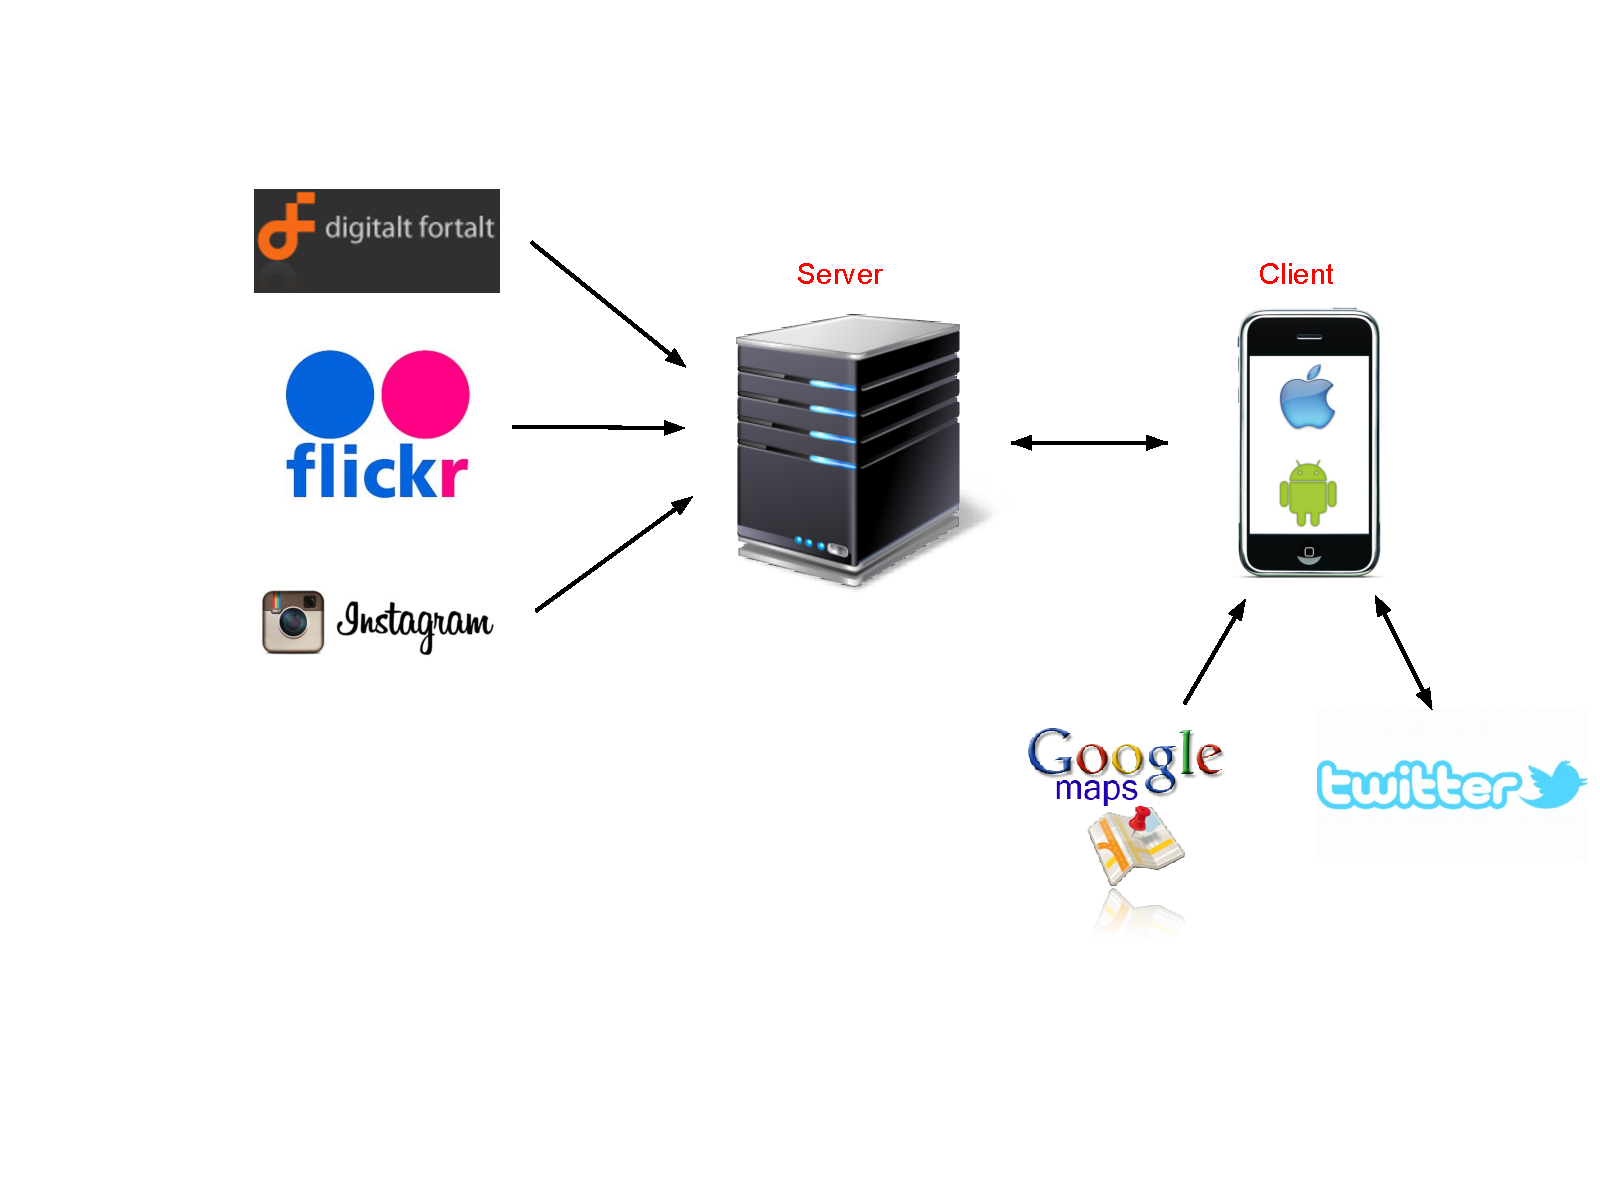
\includegraphics[scale=0.45]{ntoverview-architecture}
\caption{A simple overview of the architecture}
\end{center}
\end{figure}

\begin{itemize}
\item Browse a map and zoom in and out.
\item Load \textbf{places}.
\item Click on a place in the map and access \textbf{stories} from Digitalt Fortalt.
\item Get social media related to a place from the content providers Instagram and Twitter.
\item Go to a users exact position on a map.
\item Search for a location in the map.
\end{itemize}
	
		\subsubsection{Limitations}
There are some limitations to the system that needs to be further developed, and some that probably would require total architectural review of the project to be fixed. Our task is to continue the development of the application. An overview of the features we are going to improve are discussed in the requirements-section. Flaws that arose during the development which requires a new architecture will be discussed in the conclusions-section under Recommendations.

		\subsubsection{App evaluation}
		
After the first meetings we concluded that the best way to proceed is to evaluate the existing system, to uncover potential issues and flaws.
Therefore we decided that everyone should individually do a usability test when exploring the app for the first time. Here are a short summary of all our reports:

When opening the application the first major issue most of us experience is how slow the app loads, with little feedback that something is actually working in the background. Another thought that generally comes to mind is \emph{I don't understand the apps function when opening it without prior knowledge}. What happens is that you get a map with tags you could click on, making you believe the apps function is to bring it when visiting a town (not Trondheim in particular) and want to explore historical monuments and get Wikipedia like facts. When clicking on tags you get to the location-specific page, and there are displayed content from Instagram. Some of us found this social feature not to have very obvious intentions, it can seem like there is added social interactions to the applications just because it is popular. You would want actual and useful information about the places to be the first thing displayed and get confused when suddenly a lot of Instagram photos with random people posing with the attraction appear. Our first impression is that this social part have to offer something more interesting to be relevant at this point. There is added a nice touch with a slight gradient to white i the bottom indicating that you can scroll down for more content. When the phone is turned (switched to landscape mode) there are issues however, there are no scroll function here limiting the content available and the images are cropped. Also if there is lot of text added in the Instagram feed, this and hash-tags disappears. The way to collect images from Instagram to the application also seems to be less than optimal when sometimes completely irrelevant content are displayed. When tweeting there are no limitations on length, which causes problems when trying to post tweets over 140 characters.\\
These are some of the feedback extracted from the individual tests. 

		
	\subsection{Survey}


	One of the most important research we did during the pre-study was to conduct interviews about Stedr. In these interviews we let six everyday people, use the current version of Stedr and paid close attention to how they used it. The subjects was both male and female raging between 18-30 in age. The main purpose of this interview session was to get feedback on proposed features from our customer.\\*[8pt]
	Firstly, after the test subject had some time to play with the app. We asked asked some questions about social media integrations, and this is the results:\\

	\emph{Can you see yourself tweeting about a place from Stedr?}\\
	Yes: \textbf{0}\hspace{0.5cm}
	No: \textbf{3}\hspace{0.5cm}
	Don't know: \textbf{3}\\[6pt]
	
	\emph{What about Instagram?}\\
	Yes: \textbf{0}\hspace{0.5cm}
	No: \textbf{3}\hspace{0.5cm}
	Don't know: \textbf{3}\\[6pt]
	
	\emph{What about SoundCloud?}\\
	Yes: \textbf{0}\hspace{0.5cm}
	No: \textbf{4}\hspace{0.5cm}
	Don't know: \textbf{2}\hspace{0.5cm}\\[6pt]

	Additionally, we asked about Wikipedia. This was a proposition from us.\\*[8pt]
	\emph{Would you like the app better if Wikipedia was integrated?}\\
	Yes: \textbf{6}\hspace{0.5cm}
	No: \textbf{0}\hspace{0.5cm}
	Don't know:  \textbf{0}\\*[8pt]
	In retrospect, we see that even though people were positive to this, it doesn't really fit into what Stedr is about. Because of this, we abounded this feature late on.\\
	
	When asked if they can envision using the app in the future, this was their responses:
\begin{itemize}
	\item ”Yes, if the app can also show patios.”
	\item ”Unfortunately, I don't use social media that much, but if the app was more historically oriented, I would be intrigued to use it.”
	\item ”Yes totally!”
	\item ”It must be better than Google Maps for me to bother using it. I want the social features, but only for contributing, not for looking at what other people write. I would also use twitter with the app, but only if there was pre defined tweets.”
	\item”Maybe, if I knew about it.”
	\item ”Yes, it sounds like a good idea.”
\end{itemize}

	The general consensus was very positive about Stedr. Everyone liked the idea, but some were sceptical in regards to the social features that was purposed.

	In response to these results, our customer thought this survey was helpful, but it didn't change her mind because she had previously organized focus groups with other results. She still wanted us to integrate Stedr with SoundCloud, even though the user feedback wasn't positive about this feature. We of course respect this decision, but we felt it was our duty to do this research anyway.
	
	\subsection{Tools and technologies}
	
		\subsubsection{APIs}
		
		There was a wish from the customer that we should use other existing services as mush as possible instead of having our own database and a comprehensive back-end. The result of this is that the project will be dependent on many different APIs to function properly. As a result of this we spent alot of time researching different APIs. The existing system had already Norvegiana, Flickr, Instagram and twitter, though some of them needed a fresh up. In addition our both us and our customer had ideas to expand functionality which meant more APIs. We did research on a lot of different APIs, many of them we ended up not using, among them Google Places, Wikipedia, NRK. 
		
\paragraph{Digitalt Fortalt and Norvegiana.}

After an evaluation in the pre-study phase we decided to switch the main API the application is using for better performance. Here are a short summary of why:

In current condition, Stedr uses an API called Norvegiana. This API is basically a collection of all public APIs that can be used in collecting different data. The major pros using Norvegiana are the portion of information accessible from different sources including \emph{Statsarkivet, Digitalt Fortalt, Digitalt Museum} etc. There are many filtering options making Norvegiana able to return all the information needed.

There has been some complaints about how the current service works. Norvegiana is an interface to the dissemination system, not the production system. Which means that when a story is created, one has to wait for the Art Council Norway to perform an export from production to dissemination. This means that stories are not available through Norvegiana at once after they are produced. In some case we had to wait a few weeks. This is not acceptable with respect to our goal of increasing user participation. We think this problem might be solved by switching completely to the Digitalt Fortalt API, which should not be too much trouble considering the existing code only makes simple calls to the API trough Norvegiana. It is worth noting though that Digitalt Fortalt is originally meant for Norwegian cultural heritage, which might cause problems in a potential international expansion.

The functionality in the APIs, for our usage, are about the same. Where both come short is that both strictly speaking work like databases that you only can retrieve information from, making them impossible to use for posting new content. This has to be solved in another way.

	\subsection{Similar products}
		
A natural part of the pre-study was to explore the market for systems providing similar services. Though we did not find any identical products in terms of purpose and execution, there were a lot of products with some similar functions. 

\todo{Jørgen}

